\linespread{1.3}
\section{Задание 5. Ряд Фурье}
\subsection{Задание}
С помощью разложения в ряд Фурье данной функции в интервале  найдите сумму указанного числового ряда. Изобразите графически три различные частичные суммы разложения функции в ряд Фурье, взяв первые несколько слагаемых ряда, а также исходную функцию.\\
\begin{equation*}
	f(x) = 1 - x^2, \quad \sum_{n=4}^\infty (-1)^{n + 1} \frac{1}{(n - 2)^2}
\end{equation*}
\begin{flalign*} 
	&\text{Функция периодичная и четная, ряд Фурье будет иметь вид:}&&\\
	&f(x) = \frac{a_0}{2} + \sum_{n=1}^\infty a_n \cos nx, b_n = 0&&\\
	&a_0 = \frac{1}{\pi} \int_{-\pi}^\pi f(x)dx =  \frac{2}{\pi} \int_{0}^\pi f(x)dx =  \frac{1}{\pi} \int_{-\pi}^\pi (1 - x^2) dx = \frac{6 - 2\pi^2}{3}&&\\
	&a_n = \frac{1}{\pi} \int_{-\pi}^\pi f(x) \cos nx dx =  \frac{2}{\pi} \int_{0}^\pi (1 - x^2) \cos nx dx = \frac{2}{\pi n} \sin x \bigg |_0^\pi - \frac{2}{\pi}\int_0^\pi x^2 \cos nx dx = &&\\
	&u = x^2, du = 2xdx &&\\
	&dv = cosnxdx, v = \frac{1}{n}\sin nx &&\\
	&= -\frac{2}{\pi} (x^2\frac{1}{n}\sin nx \bigg |_0^\pi - \int_0^\pi \frac{2x}{n} \sin nx dx) = \frac{4}{\pi n} \int_0^\pi x \sin nx dx =&&\\
	&u = x, du = dx&&\\
	&dv = \sin nx dx, v = -\frac{1}{n} \cos nx&&\\
	&= \frac{4}{\pi n} (-x \frac{1}{n} \cos nx \bigg |_0^\pi + \int_0^\pi \frac{1}{n} \cos nx dx) = -\frac{4}{\pi n} \pi \frac{1}{n} \cos \pi n = -\frac{4}{n^2} (-1)^n&&\\
	&a_0 = \frac{6 - 2\pi^2}{3}, a_n = -\frac{4}{n^2} (-1)^n&&\\
	&f(x) = 1 - x^2 = \frac{3 - \pi^2}{3} + \sum_{n=1}^\infty -\frac{4}{n^2} (-1)^n \cos nx, \text{при $x \in (-\pi; \pi)$}&&\\
\end{flalign*}
\begin{center}
	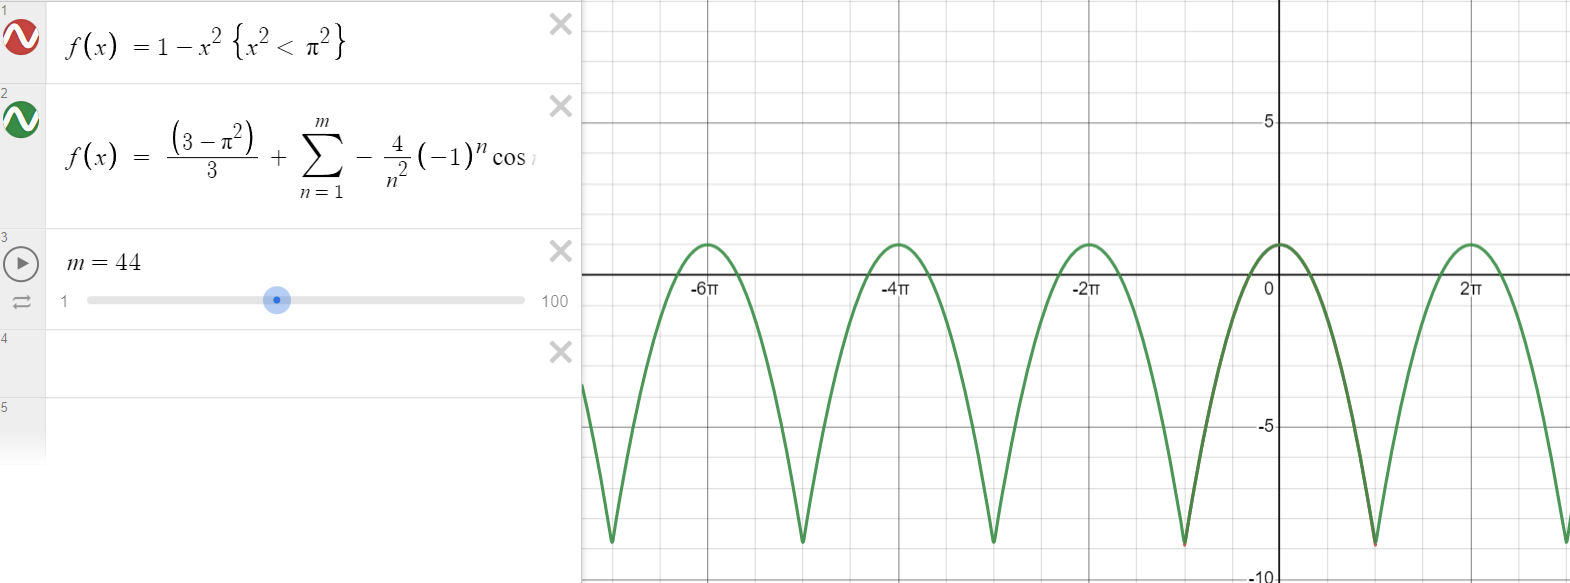
\includegraphics[width=0.9\linewidth]{task5_img1}\\
	\url{https://www.desmos.com/calculator/kbwdhz0aqe?lang=ru}
\end{center}
\begin{flalign*}
	&\text{рассмотрим x = 0:}&&\\
	&1 - 0 = \frac{3 - \pi^2}{3} + \sum_{n=1}^\infty \frac{4}{n^2} (-1)^n&&\\
	&-\sum_{n=1}^\infty \frac{4}{n^2} (-1)^n = \frac{3 - \pi^2}{3} - 1&&\\
	&-\sum_{n=1}^\infty \frac{4}{n^2} (-1)^n = -\sum_{n=3}^\infty \frac{4}{(n - 2)^2} (-1)^n = 4\sum_{n=3}^\infty \frac{1}{(n - 2)^2} (-1)^{n+1} = 4 + 4\sum_{n=4}^\infty \frac{1}{(n - 2)^2} (-1)^{n+1}&&\\
	&\text{Тогда искомый ряд:}&&\\
	&\sum_{n=4}^\infty \frac{1}{(n - 2)^2} (-1)^{n+1} = \frac{\frac{3 - \pi^2}{3} - 1 - 4}{4} = - \frac{12 + \pi^2}{12}&&\\
\end{flalign*}